\documentclass[aspectratio=169,usepdftitle=true]{beamer}

\usepackage[T1]{fontenc}
\usepackage[utf8]{inputenc}
\usepackage{microtype}
\usepackage[english]{babel}
\usepackage{lipsum}
\usepackage{multirow}
\usepackage{amsmath}
\usetheme{dividing-lines}
\usepackage{amsfonts}

\title{Impact of Covid-19 pandemic in health services usage}
%\subtitle{This is madness}
\institute{UB School of Economics Young Research Meeting}
\license{\ccbysa}

\date{September 22nd 2022}

\author{David Mori\~na, Amanda Fern\'andez-Fontelo, Pere Puig and Montserrat Guill\'en}
\email{dmorina@ub.edu}

\outro{Thank you!}
\titleimage{\tikz\node[opacity=.45]{
\includegraphics[width=4cm,height=\height,keepaspectratio]{BUlogo_cmyk-eps-converted-to.pdf}};}

% just an example command
\newcommand\twosplit[3][t]{%
\begin{columns}[#1]
\begin{column}{0.475\linewidth}#2\end{column}\hfill
\begin{column}{0.475\linewidth}#3\end{column}
\end{columns}}

\usepackage[backend=bibtex8,style=alphabetic]{biblatex}
%\addbibresource{example.bib}
\begin{document}

\section{Presentation}
\begin{frame}{Who?}
%\vspace{-1.7cm}
%  \includegraphics[height=1.7cm,width=1.7cm]{foto_simpson.jpg}
\begin{itemize}
  \item PhD in Mathematics, Universitat Autònoma de Barcelona, 2013 (New models for discrete time series)
  \item Department of Econometrics, Statistics and Applied Economics
  \item Riskcenter-IREA 
\end{itemize}
\end{frame}

\section{Problem}
\begin{frame}{Why?}
\begin{itemize}
 \item There is an enormous global concern around 2019-novel coronavirus (SARS-CoV-2)
infection in the last months, leading the World Health Organization (WHO) to declare
public health emergency in early 2020
 \item The consequences derived from the pandemic
caused by this virus have had a profound effect on many areas of human activity
 \item In addition to the direct consequences, in 2020 a decrease in use of health services has been detected, both those belonging to the Public Health System and services associated with private health insurances
\end{itemize}
\end{frame}

\begin{frame}{Why?}
\begin{itemize}
 \item The question is to know if, either due to the effect of
postponing visits or due to the consequences of having suffered the virus (persistent Covid
or secondary effects), there will be an excess of claims in 2022 and the following years
 \item There is already evidence of a higher frequency of use of Health services in the Public
System but it is difficult to determine if the highest frequency of
claims that will be observed will be equal to or greater than the infra-loss rate that was
observed during the pandemic period
\end{itemize}
\end{frame}

\begin{frame}{Why?}
\hspace{-0.9in}
  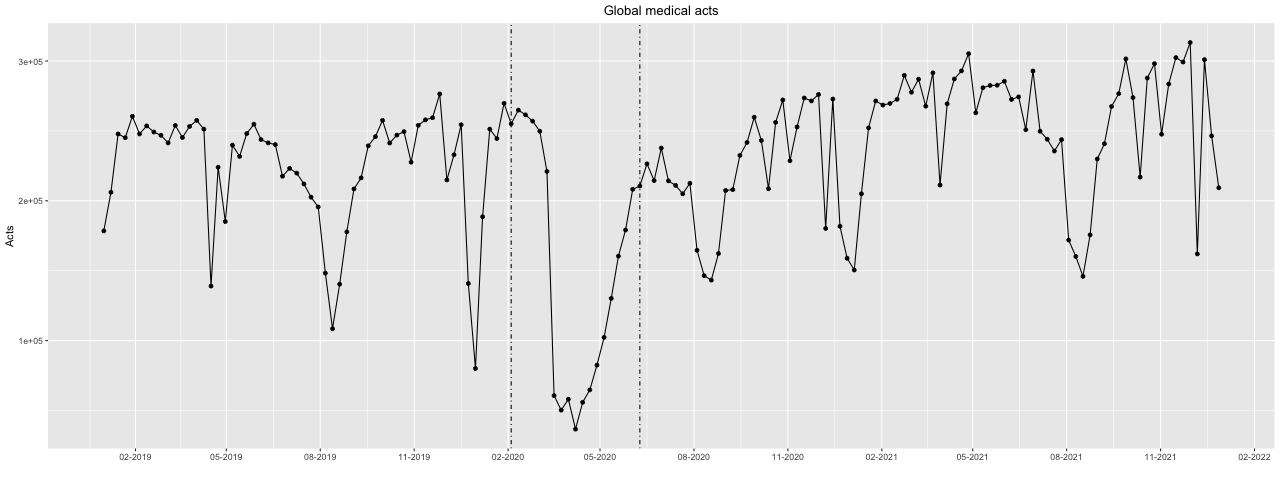
\includegraphics[height=6.5cm,width=13cm]{global_acts.png}
\end{frame}

\section{Proposed model}
\begin{frame}{How?}
\begin{center}
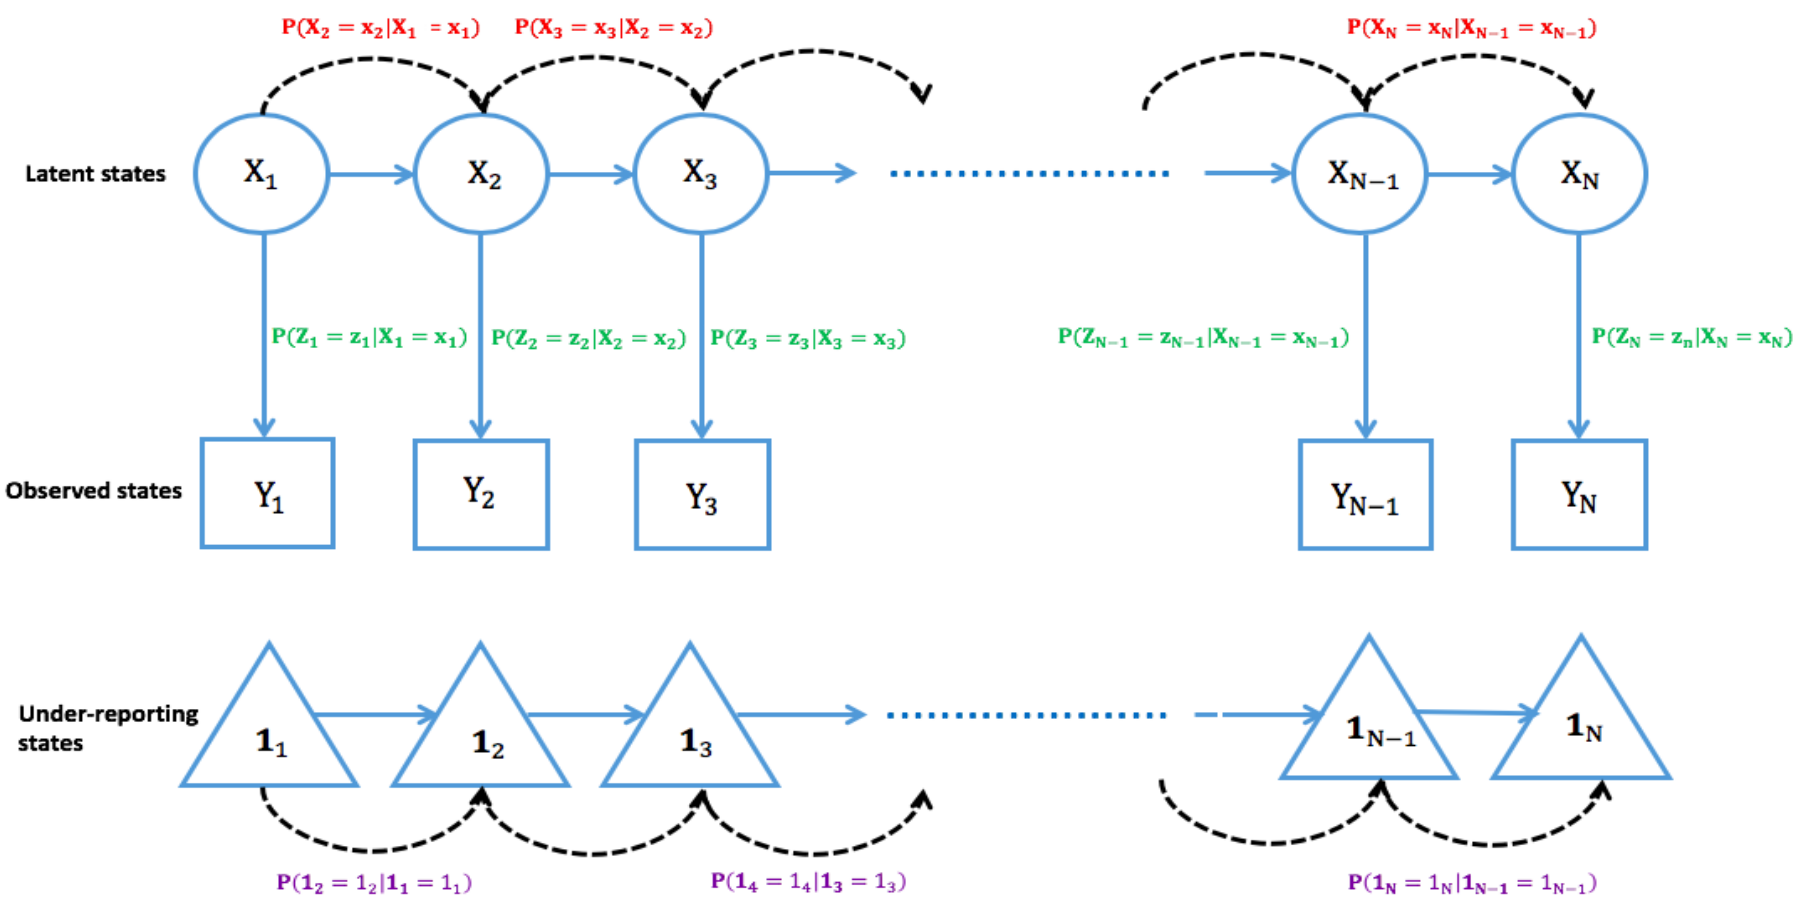
\includegraphics[height=6cm,width=11cm]{HMC.png}
\end{center}
\end{frame}

\begin{frame}[c]{Previously proposed models}
    \begin{block}{Independent under-reporting states}
        \begin{center}
           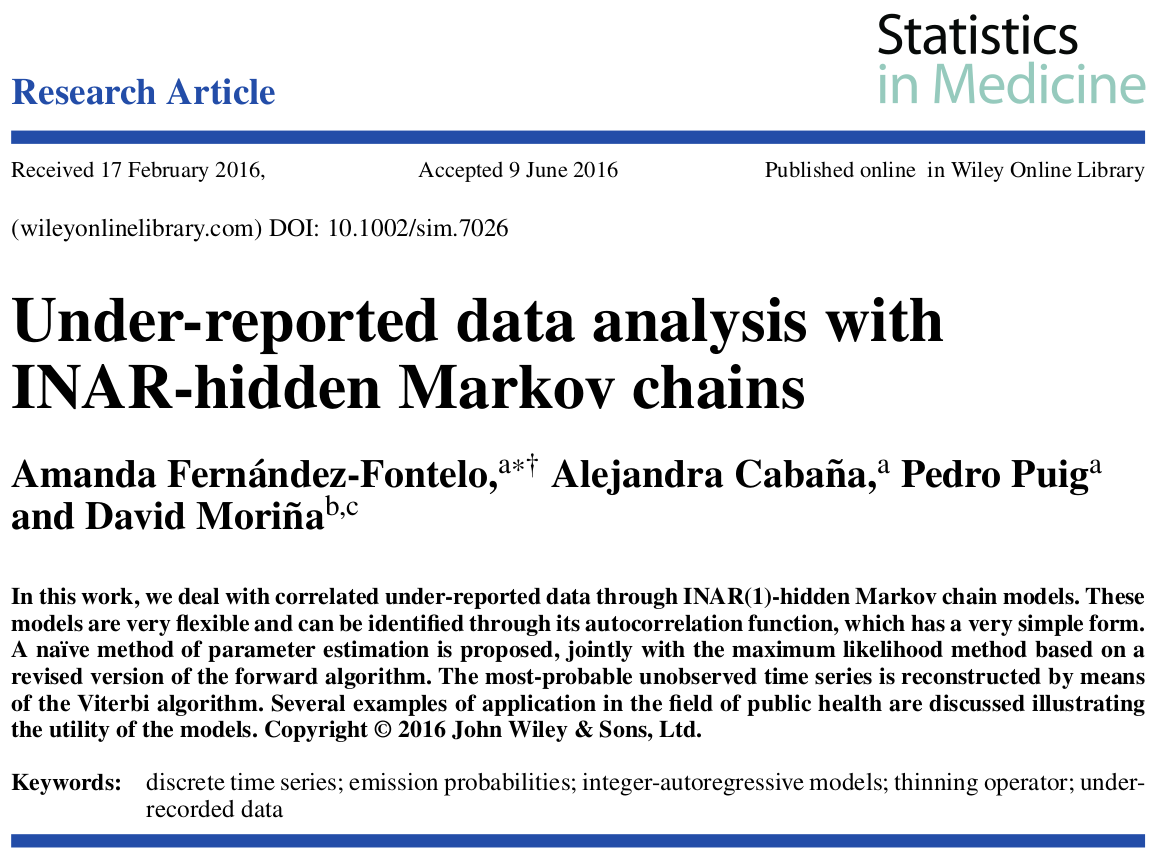
\includegraphics[height=4.7cm,width=7.5cm]{SiM1.png}
        \end{center}
    \end{block}
\end{frame}

\begin{frame}[c]{Previously proposed models}
    \begin{block}{Serially dependent under-reporting states}
        \begin{center}
           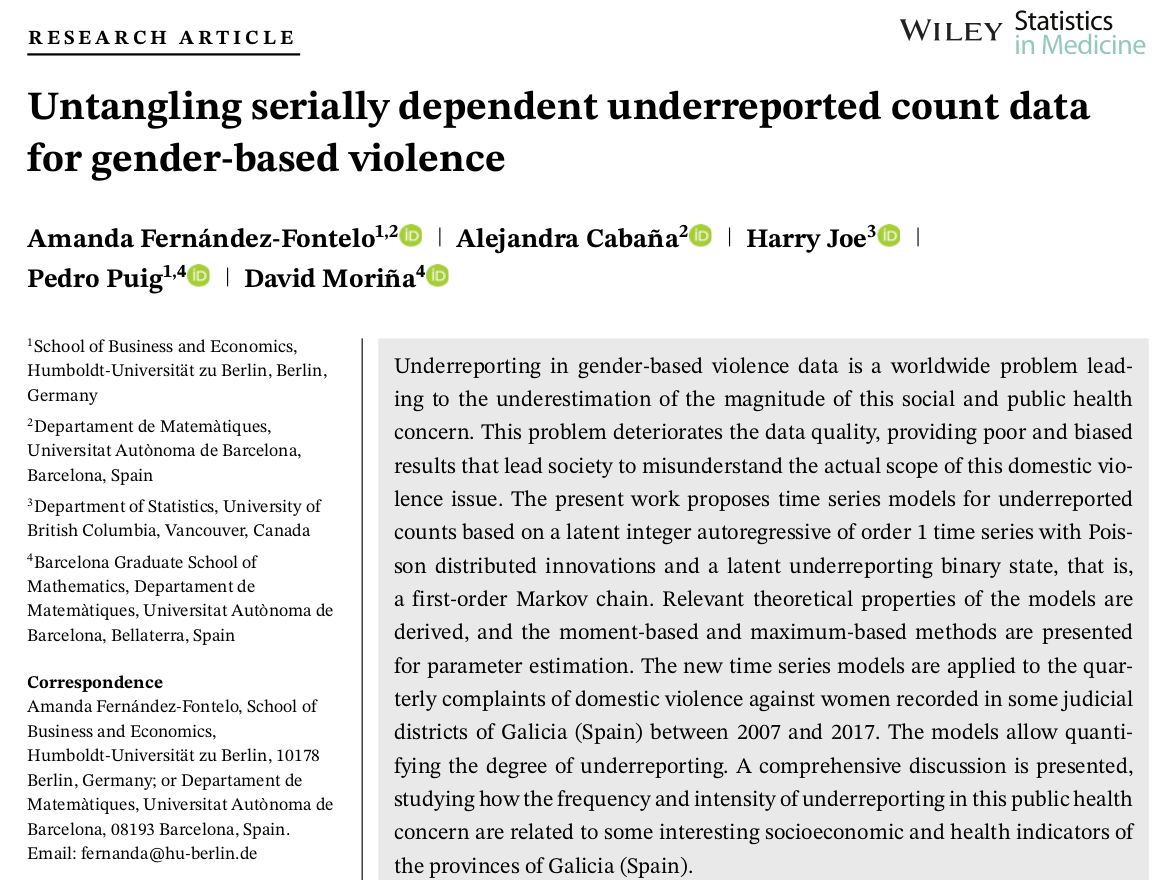
\includegraphics[height=4.7cm,width=7.5cm]{SiM2.png}
        \end{center}
    \end{block}
\end{frame}

\begin{frame}[c]{Previously proposed models}
    \begin{block}{Non-stationary processes}
        \begin{center}
           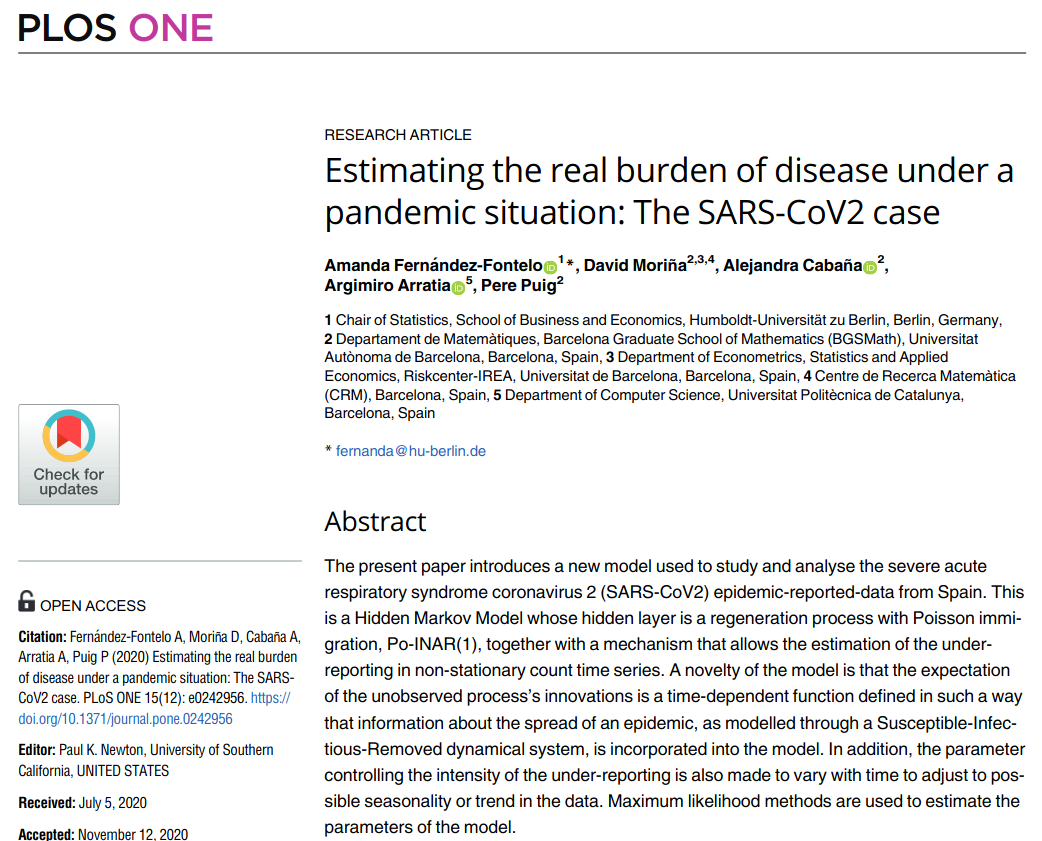
\includegraphics[height=4.7cm,width=7.5cm]{Plos.png}
        \end{center}
    \end{block}
\end{frame}

\end{document}